\documentclass[__main__.tex]{subfiles}

\begin{document}

\section{Триангуляция области с липшицевой границей. P-унисольвентное множество функционалов на P. Теорема о необходимых и достаточных условиях. Конечный элемент в $\mathbb{R}^n$. Функции формы конечного элемента. Оператор P-интерполяции. Оператор табуляции в конечном элементе. Конечно-элементное пространство $X_h$ . Оператор $X_h$-интерполяции.}

\begin{definition}
Пусть $\Omega \in \mathbb{R}^n$ - область с липшицевой границей. Тогда система подмножеств $T_n \subset 2^{\Omega}$ называется \textbf{триангуляцией} $\Omega$, если 

\begin{enumerate}
	\item $\forall k \in T_n, \partial K \subset K, \mathring{K} > K\backslash\partial K \neq \varnothing$
	
	\item $\forall k_1, k_2 \in T_n, \mathring{K_1} \bigcap \mathring{K_2} = \varnothing$
	
	\item $\forall K \in T_n$, k - липшицева область
	
	\item Если $k \in T_h$- многогранник, тогда для всех его границ Г следует, что $\Gamma \subset\partial \Omega$ либо $\exists k_1 \in T_h$ $\Gamma$ - грань $k_1$, где $h = max diam k_1,$ где $k \in T_h$
	
	\begin{figure}[h!]
		\centering
		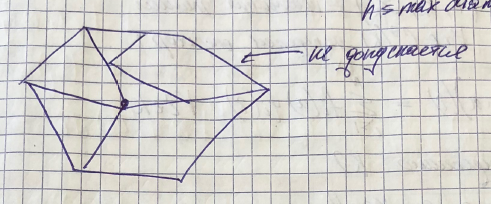
\includegraphics[width=0.7\linewidth]{screenshot002}
		\caption{}
		\label{fig:screenshot002}
	\end{figure}
\end{enumerate}
\end{definition}

\begin{definition}
Пусть P - конечномерное линейное пространство функций на липшицевой области $\Omega$. Тогда конечное множество функционалов $\Sigma = \{f_i, i = 1 ... N\}$ на P называется \textbf{P - унисротвентными}, если $\forall \alpha_i \in R$, i = 1...N $\exists! p\in P$, что $f_i\left(p\right) = \alpha_i, i = 1...N$.
\end{definition}

\begin{theorem}
	Множество $\Sigma$ - P - унисольвентно тогда и только тогда, когда 
	
	\begin{enumerate}
		\item $dim P = \left|\Sigma\right|$
		
		\item  $\exists \varphi_i \in P, i = 1... N$ что $f_i \left(\varphi_j\right) = \delta_{ij}$, $i,j = 1 ...N$
	\end{enumerate}
\end{theorem}

\begin{definition}
Пусть К - ограниченное множество в $\mathbb{R}^n$, $P_k$ - (множесттво линейных функционалов на К) конечномерное линейное пространство функций на К, $\Sigma_K = \{f_i, i = 1 ... N\}$ - конечное множество функционалов на $P_K$

\begin{enumerate}
	\item K - липшицева область, $\partial K \subset K, \mathring{K} = K \backslash \partial K$ 
	
	\item  $\exists s \in Z_+:P_K \subset C^s\left(K\right)$
	
	\item $\Sigma_K - P_k$ - унисольвентное множество и $f_i, i= 1...N, f_i:C^s\left(\Omega\right) \rightarrow \mathbb{R}$ .
\end{enumerate}

Тогда \textbf{конечный элемент} - это тройка $\left(K, P_k,, \Sigma_K\right)$
\end{definition}

\begin{definition}[Оператор интерполяции]
	Пусть $\left(K, P_K, \Sigma_K\right)$ - конечный элемент. Тогда $\forall x \in C^s\left(K\right)$ определён оператор:
	
	$$
	\left(\Pi_k \circ x\right) \left(\tau\right) = \sum_{i = 1}^{N}f_i\left(x\right)\varphi_i\left(\tau\right), \forall \tau \in K
	$$
	
	По определению КЭ
	
	$\Pi_k \circ p = p, \forall p \in P_k$
\end{definition}

\begin{definition}[Оператор табуляции]
	Пусть $\left(K, P_k, \Sigma_K\right)$ - КЭ. Тогда оператор $T_k: C^s\left(\Omega\right) \rightarrow \mathbb{R}^N$  - оператор табуляции, если 
	
	$$
	T_K \left(x\right) = 
	\left(
	\begin{matrix}
	f_1\left(x\right) \\
	... \\
	f_n\left(x\right)
	\end{matrix}
	\right)
	$$
	
	Если $\left(K, P, \Sigma_K\right)$ - КЭ, то оператор интерполяции записывается в виде:
	
	$$
	\Pi_k \circ x = \sum_{i = 1}^{n} f_i\left(x\right) \varphi_i = \varphi^T \circ T_K\left(x\right),
	$$
	
	где $\varphi\left(\tau\right) = \left(\begin{matrix}
	\varphi_1\left(\tau\right) \\
	... \\
	\varphi_n \left(\tau\right)
	\end{matrix}\right)$
\end{definition}

\begin{definition}[Множество узлов триангуляции $T_n$]
	Пусть $T_n$ -триангуляция $\Omega$. Тогда конечное множество точек $N_n$ из $\Omega$ - множество узлов $T_h$, если $\forall K \in T_h \exists x \in N_n$, что $x \in \partial K$.
\end{definition}

\begin{definition}[Конечно - элементное пространство]
Пусть $\left(K, P_k, \Sigma_K\right)$ - семейство КЭ соответствующих триангуляции $T_h$. Тогда множество $x_h$ - КЭ пространство, если 

$$
x_h = \{x: x\big|_K P_K, \forall K \in T_h, \left(x\big|_{K_1}\right)\left(a\right) = \left(x\big|_{K_2}\right)\left(a\right) \forall a \in N_n: a\in K_1 and a\in K_2 \}
$$
\end{definition}

\begin{definition}[Оператор интерполяции в $X_h$]
	Оператор $\Pi_h: C^s \left(\Omega\right) \rightarrow X_h$ - оператор интерполяции в $X_h$ если:
	
	$$
	\left(\Pi_h \circ x\right)\big|_K = \Pi_k \circ x, \forall K \in T_h
	$$
\end{definition}

\end{document}
